\begin{figure*}[!t]
\begin{minipage}{0.48\linewidth}
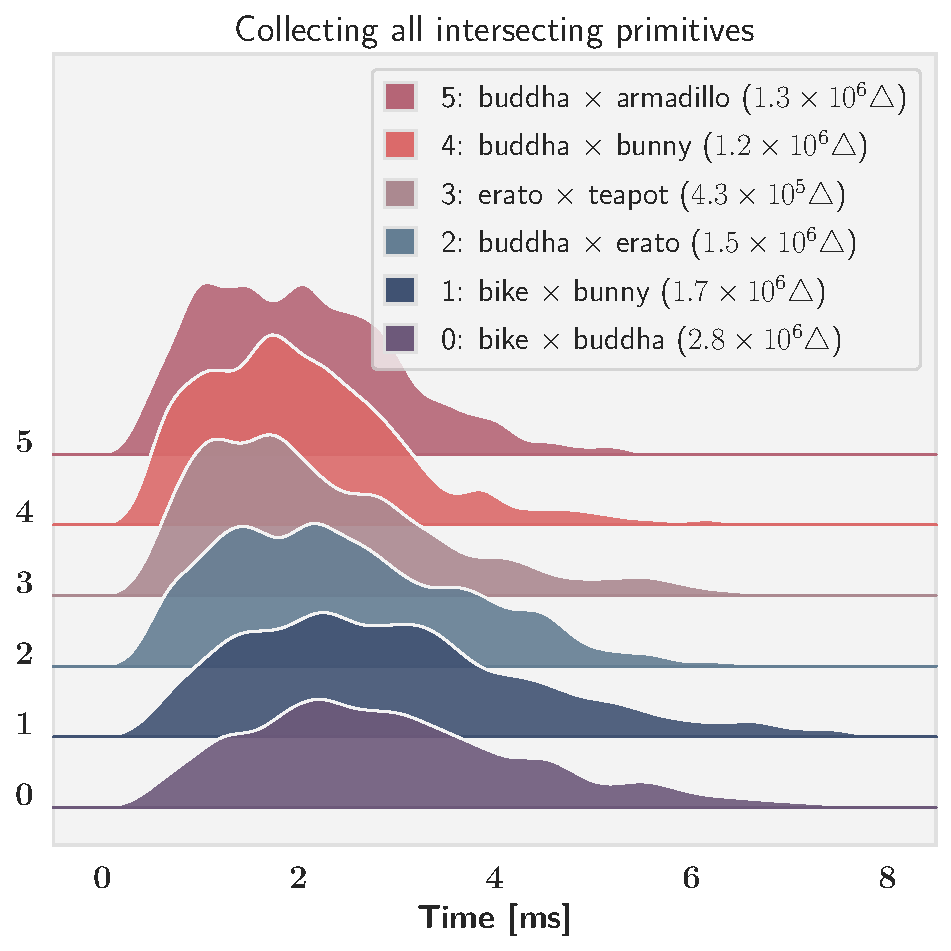
\includegraphics[width=\linewidth]{../figures/intersect-kde.pdf}
\end{minipage}
\begin{minipage}{0.48\linewidth}
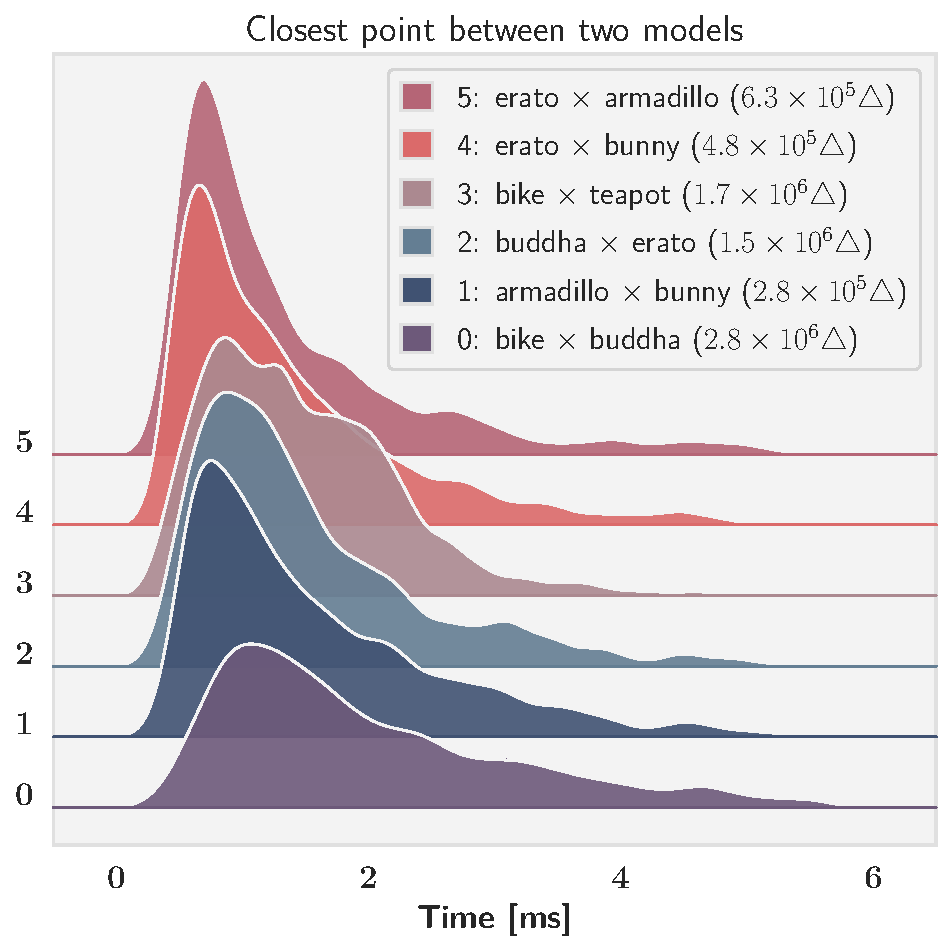
\includegraphics[width=\linewidth]{../figures/closest-kde.pdf}
\end{minipage}
\caption{
Runtime distributions for queries between two models (from Computer Graphics Archive~\cite{McGuire2017Data})
using \texttt{tf::tree} The total number of triangles per query is marked next to $\triangle$.
Each distribution was estimated
on $10{,}000$ samples of relative positions.
\textbf{Left:} Time needed to compute all intersecting
primitives between two meshes. Each sample contained
an intersecting configuration.
\textbf{Right:} Time needed to compute a pair of
closest points between the two models. Each sample
contain a non-intersecting configuration.
}\label{fig:query-dists}
\end{figure*}
